% A complete, compilable §I-P2 "paradigm-swimlanes" FRAMEWORK figure — the
% single most common shape of a method/framework hero: a mechanistic track and a
% data-driven track fused at a bridge node (the contribution). This is the figure
% a 数模/scientific paper puts on page 1 as its 技术路线图 / model framework.
%
% Build:  pdflatex framework_hero.tex   ->  framework_hero.pdf
% Paper:  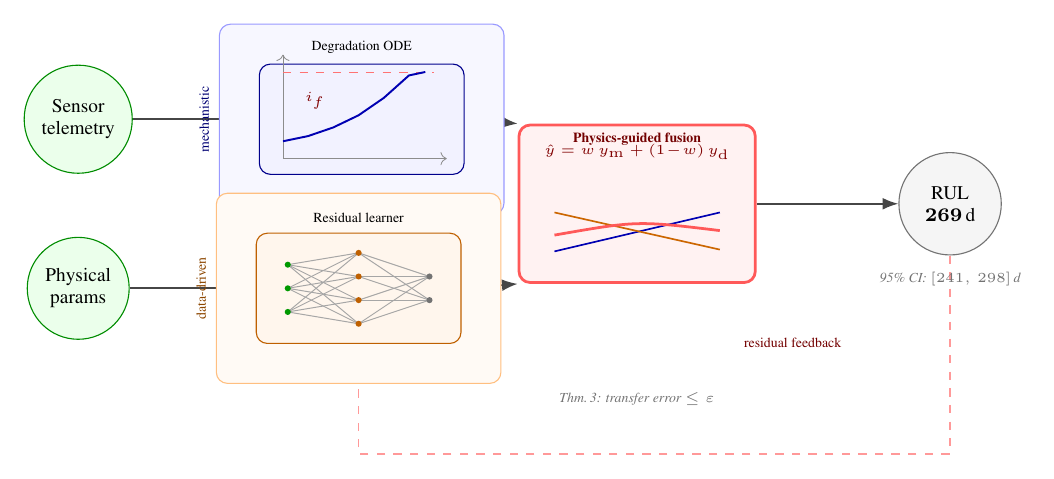
\includegraphics[width=\linewidth]{framework_hero.pdf}
%         (the main document never touches tikzpicture -> zero compile risk)
%
% It demonstrates the THREE borrowable techniques distilled in
% references/framework-figures.md (adapted from tikz.net / Izaak Neutelings):
%   (1) colour-coded semantic nodes  (input=green, process=blue/orange by lane,
%       hero=red, output=grey) so input/process/output read at a glance;
%   (2) connections drawn on a BACKGROUND layer so a dense framework stays clean;
%   (3) trapezoid/fit GROUPING boxes that turn loose blocks into named "lanes".
% And the §0b axis-1 rule: each lane embeds a REAL method object (a degradation
% curve; a small network), not the words "mechanistic" / "neural net".
\documentclass[tikz,border=3mm]{standalone}
\usepackage{times}
\usetikzlibrary{positioning, arrows.meta, fit, backgrounds, shapes.geometric, calc}
\begin{document}
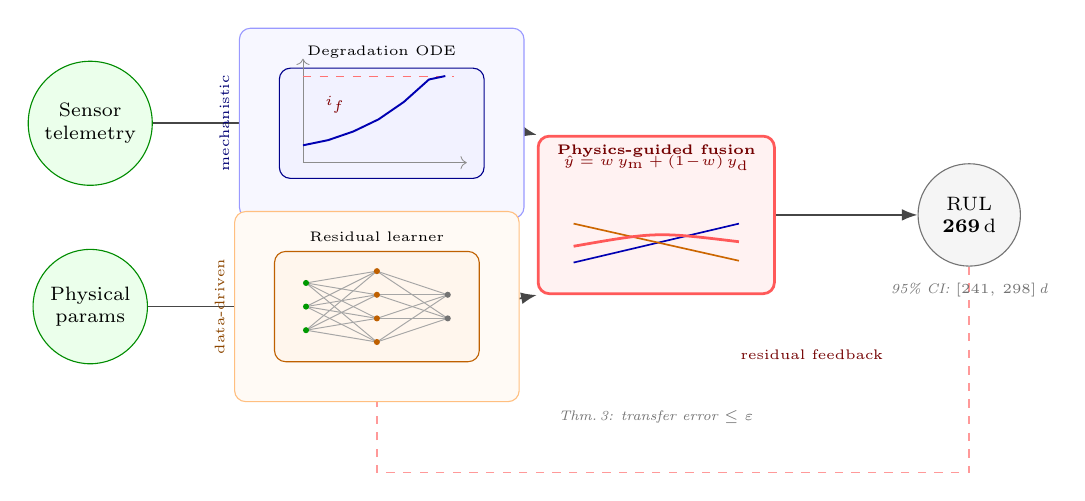
\begin{tikzpicture}[
  % --- technique (1): one style per SEMANTIC role, colour encodes the role ------
  io/.style    = {circle, draw=green!55!black, fill=green!8, minimum size=12mm,
                  align=center, font=\scriptsize},
  mech/.style  = {rectangle, draw=blue!55!black, fill=blue!5, rounded corners,
                  minimum height=14mm, minimum width=26mm, align=center, font=\scriptsize},
  data/.style  = {rectangle, draw=orange!75!black, fill=orange!7, rounded corners,
                  minimum height=14mm, minimum width=26mm, align=center, font=\scriptsize},
  hero/.style  = {rectangle, draw=red!65, line width=1pt, fill=red!5, rounded corners,
                  minimum height=20mm, minimum width=30mm, align=center, font=\scriptsize},
  result/.style= {circle, draw=black!55, fill=black!4, minimum size=13mm,
                  align=center, font=\scriptsize},
  arr/.style   = {-{Latex[length=2mm]}, semithick, gray!55!black},
  thm/.style   = {font=\tiny\itshape, text=black!55},
]
  % ============================ INPUT (left) ================================== %
  \node[io] (sens) {Sensor\\telemetry};
  \node[io, below=8mm of sens] (phys) {Physical\\params};

  % ===================== MECHANISTIC LANE (top, blue) ========================= %
  % real object: a degradation curve i(t) crossing a failure threshold ---------
  \node[mech, right=16mm of sens] (mechb) {};
  \node[font=\tiny, anchor=south] at (mechb.north) {Degradation ODE};
  \begin{scope}[shift={($(mechb.center)+(-10mm,-5mm)$)}, x=1.6mm, y=2.2mm]
    \draw[->, black!45, line width=0.3pt] (0,0) -- (13,0);          % t axis
    \draw[->, black!45, line width=0.3pt] (0,0) -- (0,6);           % i axis
    \draw[red!55, dashed, line width=0.3pt] (0,5) -- (12,5);        % i_f threshold
    \node[font=\tiny, text=red!50!black, anchor=north west] at (1,4.4) {$i_f$};
    \draw[blue!70!black, line width=0.7pt]                          % i(t)=i0+a(e^{bt}-1)
      plot coordinates {(0,1)(2,1.3)(4,1.8)(6,2.5)(8,3.5)(10,4.8)(11.3,5)};
  \end{scope}

  % ===================== DATA-DRIVEN LANE (bottom, orange) ===================== %
  % real object: a 3-layer network drawn with technique (2) loop-based placement -
  \node[data, right=16mm of phys] (datab) {};
  \node[font=\tiny, anchor=south] at (datab.north) {Residual learner};
  \begin{scope}[shift={($(datab.center)+(-9mm,0)$)}, every node/.style={}]
    \foreach \L/\n/\c in {0/3/green!60!black, 1/4/orange!75!black, 2/2/black!55}{
      \foreach \i in {1,...,\n}{
        \coordinate (N-\L-\i) at (\L*9mm, {(\i-(\n+1)/2)*3mm});
      }
    }
    % edges first, then nodes overlay them (within a FILLED box the background
    % layer is hidden by the fill — so draw edges in-layer, dots on top)
    \foreach \i in {1,...,3}\foreach \j in {1,...,4}
      \draw[black!35, line width=0.35pt] (N-0-\i) -- (N-1-\j);
    \foreach \i in {1,...,4}\foreach \j in {1,...,2}
      \draw[black!35, line width=0.35pt] (N-1-\i) -- (N-2-\j);
    \foreach \L/\n/\c in {0/3/green!60!black, 1/4/orange!75!black, 2/2/black!55}
      \foreach \i in {1,...,\n}
        \fill[\c] (N-\L-\i) circle (1.1pt);
  \end{scope}

  % ============================ HERO: the FUSION ============================== %
  % the bridge where the two paradigms meet — embed the real fusion object
  % (a weighting w blending the two predictions), not the word "fusion" ---------
  \node[hero, right=20mm of $(mechb)!0.5!(datab)$] (fuse) {};
  \node[font=\tiny\bfseries, anchor=north, text=red!45!black] at (fuse.north) {Physics-guided fusion};
  % equation pinned under the title; prediction lines confined to the lower half
  % so the two never overlap
  \node[font=\tiny, text=red!50!black] at ($(fuse.north)+(0,-3.6mm)$)
        {$\hat y=w\,y_{\mathrm{m}}+(1\!-\!w)\,y_{\mathrm{d}}$};
  \begin{scope}[shift={($(fuse.center)+(0,-2.6mm)$)}, x=1.5mm, y=1.15mm]
    \draw[blue!70!black, line width=0.6pt] (-7,-3) -- (7,1.3);        % mech prediction
    \draw[orange!80!black, line width=0.6pt] (-7,1.3) -- (7,-2.8);    % data prediction
    \draw[red!65, line width=1pt] (-7,-1.2) .. controls (0,0.4) .. (7,-0.7); % fused
  \end{scope}

  % ============================ OUTPUT (right) ================================ %
  \node[result, right=18mm of fuse] (rul) {RUL\\$\mathbf{269}$\,d};

  % ============================ CONNECTIONS (bg) ============================== %
  % technique (2): all edges on the background layer -> nodes stay crisp on top
  \begin{scope}[on background layer]
    \draw[arr] (sens) -- (mechb);
    \draw[arr] (phys) -- (datab);
    \draw[arr] (mechb.east) -- (fuse.north west);
    \draw[arr] (datab.east) -- (fuse.south west);
    \draw[arr] (fuse) -- (rul);
    \draw[arr, dashed, red!40] (rul.south) |- ($(datab.south)+(0,-14mm)$) -| (datab.south);
  \end{scope}
  \node[font=\tiny, text=red!45!black, anchor=south] at ($(rul.south)+(-20mm,-13mm)$) {residual feedback};

  % ===================== technique (3): grouping lane boxes ==================== %
  \begin{scope}[on background layer]
    \node[fit=(mechb), draw=blue!40, fill=blue!3, rounded corners, inner sep=5mm,
          label={[font=\tiny, text=blue!45!black]left:\rotatebox{90}{mechanistic}}] {};
    \node[fit=(datab), draw=orange!50, fill=orange!4, rounded corners, inner sep=5mm,
          label={[font=\tiny, text=orange!55!black]left:\rotatebox{90}{data-driven}}] {};
  \end{scope}

  % ===================== guarantee band (anchors theory) ====================== %
  \node[thm] at ($(datab.south -| fuse)+(0,-7mm)$) {Thm.\,3: transfer error $\le \varepsilon$};
  \node[thm] at ($(rul.south)+(0,-3mm)$) {95\% CI: $[241,\,298]$\,d};
\end{tikzpicture}
\end{document}
